\chapter{Introduction}
\begin{flushright}
\emph{I am an enthusiast, but not a crank in the sense that I have some\\
pet theories as to the proper construction of a flying machine. I wish to\\
avail myself of all that is already known and then, if possible,\\
add my mite to help on the future worker who will attain final success.}\\
--- Wilbur Wright
\end{flushright}

\begin{flushright}
\emph{Everything should be made as simple as possible, but no simpler.}\\
--- Albert Einstein (rephrased)
\end{flushright}

%\begin{flushright}
%\emph{An inventor is simply a fellow who doesn't take his education too seriously.}\\
%--- Charles Kettering 
%\end{flushright}

\begin{flushright}
\emph{When a subject becomes totally obsolete we make it a required course.}\\
--- Peter Drucker
\end{flushright}

%\begin{flushright}
%\emph{A problem well stated is a problem half-solved.}\\
%--- Charles Kettering
%\end{flushright}
\minitoc

This book describes a theory of AGI (Artificial General Intelligence) \citep*{Goertzel2007} that is still being developed.  I think the AGI problem can be decomposed into $\sim$10 computational issues and we will somehow integrate them together:

\leftskip 1cm
knowledge representation\\
fuzzy-probabilistic logic\\
deduction\\
abductive reasoning\\
inductive learning\\
pattern recognition / categorization\\
belief revision\\
memory organization\\
natural language\\
sensory processing

\leftskip 0cm
My approach is predominantly logic-based, but it also employs redundancy in knowledge representation, including sub-symbolic knowledge, and therefore is somewhat like neural networks.  Also, it may merge with neural networks at the sensory level.  This approach can be called ``neo-classical AI''.

\section{Some background of AI}

The word ``logic'' comes from \textit{logos} which can mean ``word'', ``thought'', or ``reason''.  The study of logic is the study of the \textbf{mechanisms of thinking}.  Aristotle (ca 350BC) is often credited with the first substantial study of logic, with a focus on syllogisms.  Our current system of logics was developed by people such as De Morgan (1840s), Boole (1840s), Frege (1879, \textit{Begriffsschrift}), Russell and Whitehead (1903, \textit{Principia Mathematica}), and others (including Liebniz (1670s, ``algebra of thought'') whose work remain undiscovered till the 1880s).

\textbf{Logic-based AI}\\
Thus it is not so surprising that the design of AI can be based on logic.  John McCarthy (who coined the term ``AI'' in a 1956 Darthmouth conference) was first to propose the use of \textbf{formal logic} in AI.  Herbrand (1908-1931) created a basis of provability in predicate logic.  In 1965, Robinson discovered the \textbf{resolution} method for logical inference, which enabled the creation of \textbf{logic programming} and the language Prolog (Kowalski and Colmerauer, 1970s).

\textbf{Connectionism}\\
In 1943, McCulloch and Pitts formulated a formal model of neurons, leading to Rosenblatt's Perceptron (1957), and later the computational paradigm of artificial neural networks (ANNs).  In the 1980s there was a resurgence of interests in ANNs and connectionism due to the invention of the backpropagation algorithm for multilayer perceptrons.  At this point it was recognized that connectionism has the advantages of \textbf{robustness} and \textbf{graded response}, in contrast to logic-based AI's \textbf{brittleness} and \textbf{bivalence}.

\textbf{Recent trends}
In the 1990s there was rapid development in \textbf{statistical learning}.  It was then realized that ANN learning algorithms are a special case of statistical learning.  Recent development in AI is distanced from ``GOFAI'' (Good Old-Fashioned AI) by their use of statistical learning, \textbf{sub-symbolic representations}, and \textbf{optimization methods} (computational intelligence).  Computational intelligence includes new paradigms such as evolutionary computing (drawing inspiration from sexual reproduction) and swarm intelligence (drawing from social interactions).

\section{Why logic?}
\label{sec:why-logic}

I started designing AGI using the neural network approach for a few years, until I discovered some fundamental difficulties in the NN approach, so I switched to a more logic-based one\footnote{Though my approach is not purely logic-based.}.

Logic-based AI went out of vogue beginning in the 1980s because of the advent of connectionism and later statistical learning methods.  As a result, many researchers nowadays are unfamiliar with even the basics of logic-based AI.  In order to understand my approach it is extremely important to be familiar with \textbf{first-order logic} (FOL) and to understand the difference between first-order representations and propositional ones.

\textbf{Propositional vs first-order.}  This is a typical propositional statement:\\
\hspace*{1cm} $ p \vee q \wedge r $.\\
Compare it with a typical first-order statement:\\
\hspace*{1cm} $ p(X) \vee q(X,Y) \wedge r(w(Y,Z)) $.\\
The chief distinction is the use of \emph{variables} in first-order logic, which greatly increases its expressiveness.

The vast majority of statistical learning literature assumes that the data is represented by points in a high-dimensional space.  I call this the ``spatial'' approach which includes methods like nearest neighbor, support vector machines (SVMs), principal component analysis (PCA), and artificial neural networks (ANNs).  \textit{Spatial datasets are equivalent to propositional representations.}  First-order logic is a symbolic or relational\footnote{Relational representations are a subclass of first-order representations that do not allow functors and structured terms.} approach which is qualitatively very different.  There is strong evidence that some datasets can be easily learned by relational methods but are very difficult, if not impossible, to learn with spatial methods.  (\citep*{Thornton1996}, \citep*{Thornton2000}.\footnote{He demonstrated this with the example of a ``checkerboard'' pattern of 0's and 1's that can be easily learned by a logical formula, but would be very difficult for a neural-network learner.  This is actually the age-old debate between symbolic AI and connectionism, given a new twist in the context of machine learning.} provides an interesting and detailed analysis of this issue.)

To put it more bluntly, I suspect that propositional approaches are rather useless in the logic-based AI framework (but I'd be pleasantly surprised to learn otherwise).

Notice in the figure below, that all \textbf{spatial classifiers} work by ``chopping'' the space of data points (shown in 2D here) into various regions with the use of hyper-planes (as a line in 2D) or some curved boundaries.  This is very different from how first-order logic classifies data.

\begin{figure}[H]
\centering
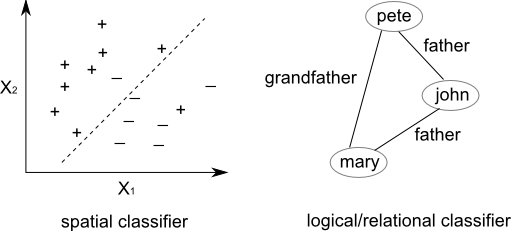
\includegraphics{spatial-vs-logical.png}
\caption{Spatial vs logical classification}
\end{figure}

To illustrate this with an example:  Let's think of how a child (AGI or human) learns the concept of (blood) relatives.  The child (Jane) would be given some examples of people around her and whether they are her relatives, eg:\\
\hspace*{1cm} father(jane, john), relative(john)\\
\hspace*{1cm} mother(jane, mary), relative(mary)\\
\hspace*{1cm} uncle(jane, pete), relative(pete)\\
\hspace*{1cm} neighbor(jane, joe), $\neg$relative(joe)\\
\hspace*{1cm} friend(jane, kate), $\neg$relative(kate)\\
and the task is to learn a general rule for relatives.  The solution can be stated quite succinctly\footnote{This solution is not entirely correct, as relatedness can grow unbounded and everyone would be ultimately blood-related.  Perhaps this problem can be resolved by fuzziness and other mechanisms such as non-monotonicity, but my point here is to show that the situation for propositional representation is even worse, as the problem appears insurmountable in that case.} in first-order logic:\\
\hspace*{1cm} relative(X, Y) $\leftarrow$ parent(X, Y)\\
\hspace*{1cm} relative(X, Y) $\leftarrow$ sibling(X, Y)\\
\hspace*{1cm} relative(X, Y) $\leftarrow$ married(X, Y)\\
\hspace*{1cm} relative(X, Y) $\leftarrow$ relative(X,Z), relative(Y,Z)\\
but it is very difficult to express in propositional logic unless we limit the domain of entities to a few people.  Also, we can see that \textit{spatial} statistical learning will fail to learn this rule because:\\
1. The dataset cannot be represented as numerical values in a vector space, or it could be done only very awkwardly.\\
2. Even when the dataset is cast in vector space, the learning algorithm can mostly learn to classify \textit{existing} examples, but the \textit{generalizations} would be wrong -- this is because the formulae in first order logic can entail discrete examples that are not necessarily located in a localized region in the numerical space.  Even if you carve the space into ridiculously complex regions, the next example would still be an exception because ``spatial compactness'' is simply absent in the underlying concept.\\
3. The child's world typically has very few people in it, yet she is able to learn the concept.  In ANNs and statistical learning, the sample size is typically at least 100s, but logic-based learning can learn the concept with just a few examples.

Although first-order representations can be converted to propositional ones via the process of propositionalization, such algorithms cost exponential time and space.  This is not difficult to see:  FOL allows us to express knowledge very succinctly.  There are some techniques that ameliorate the combinatorial explosion, such as partial instantiation (\citep*{Chandru1999}) or sparse matrix (\citep*{Domingos2008}).  But I still think it is easier and more intuitive to working on a FOL KB directly, especially for AGI.

And, despite propositionalization, the class of spatial statistical learning techniques still seem to be unsuitable for logic-based AGI because propositionalization does not cure the fundamental lack of ``compressiveness'' of predicate logic that I pointed out above.  (After propositionalization, some fast propositional SATisfiability algorithms can be invoked, but they are still qualitatively different from the spatial learning algorithms.)  From this consideration, my current strategy is to focus on algorithms specifically for FOL / HOL / predicate logic.

The application of kernel methods to logic seems to rely on syntactic distance rather than \textit{semantic} distance.  (Eg: \citep*{Muggleton2005} developed a support-vector ILP method;  \citep*{Gartner2008} describes a method that constructs kernels for (first-order and higher-order) logic formulae, based on a representation of logic by typed lambda calculus in \citep*{Lloyd2003}.  It involves the use of a ``matching kernel'' that measures syntactic distance only.)  So far I have not seen an effective way to estimate semantic distance without performing logical inference.

\{ Some new techniques have been developed to lift neural networks to first-order representations, but I have not examined them in detail (eg, \citep*{Garcez2009}, \citep*{Hammer2007}).  \}

\{ To-do:  I've gained some new insight into the issue of mapping predicate logic to continuous space, via algebraic logic. \}

\section{Why not neural network?}

There are several reasons why I think the NN approach may be less promising:

1.  First-order logic is a more powerful representation scheme than (feed-forward) neural networks (\S\ref{sec:why-logic}), whereas dynamic neural networks are very difficult to work with.

2.  A neuron is "fixed" within a network and cannot "move around", which seems to make it difficult to perform invariant pattern recognition (eg, translational, rotational, and scale- invariance in vision). The brain has to use neurons due to biological constraints, but it seems more effective to use other pattern matching methods on von Neumann machines. (Scale invariance is particularly difficult for ANNs, see \citep*{Muresan2004}.)

3.  Neural learning is slower and require a larger amount of examples. Logic-based learning is coarse-grained and thus require fewer examples to induce the correct representation, sometimes as few as 1 example.

4.  As Ben Goertzel pointed out some years ago, a network of redundant propositions can be reduced to a minimum number of non-redundant propositions, without loss of information;  the only thing that is lost is \textit{fault tolerance}.

However, neural networks may be used for handling low-level vision, especially at the feature-extraction level.

\section{Recursive self-improvement}
\label{sec:RSI}

RSI refers to the ability of an AGI to reprogram itself.  Some authors predict that the RSI point will trigger the Technological Singularity (eg \citep*{Kurzweil2005}).  I think the way to reach the RSI point with the least amount of efforts would be to build an automatic program synthesis tool that accepts natural-language commands or goal specifications.  From then on, we can use this tool to rewrite the tool itself and to evolve it (semi-automatically) into a full AGI system.

\section{Chicken-and-egg problem}
\label{sec:chicken-and-egg}

\begin{figure}[H]
\centering
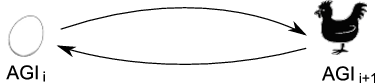
\includegraphics{chicken-and-egg1.png}
\caption{chicken and egg problem}
\end{figure}
\vspace{-0.5cm}

Anyone who has thought about AGI long enough will be aware of this problem:  The idea is to use a ``program evolver'' that takes an input program $\Pi_i$ and improves it to $\Pi_{i+1}$ according to some user-specifications.  We put the evolver through itself, thus building up its intelligence recursively without doing any programming (except for the initial evolver).

This idea (at least naively) does not work because the initial evolver needs to have very good background knowledge about programming or else it cannot perform its job in reasonable time.  \S\ref{sec:self-programming-architecture} discusses how to make it feasible.

\section{Natural reasoning}
\label{sec:natural-reasoning}

Other names for natural reasoning are: common-sense reasoning, human-like reasoning, informal reasoning.

Natural reasoning is an extension of logical reasoning with:\\
1.  ability to recognize natural concepts (which I posit requires fuzzy pattern recognition)\\
2.  ability to use metaphors, similes, analogies, and similarity-based reasoning

An example of natural reasoning is:

\leftskip 1cm \textit{Suppose I need to write a program to ``break English sentences into words''.  I'd need to declare a function to do this.  What would be the input and output of this function?}

\leftskip 0cm Note that in the above reasoning, I think of the function as a ``box'' with something that goes in and something out.

Natural reasoning is required to turn informal, natural-language statements into formal statements.  This is especially important to formal program synthesis.
